\documentclass[11pt,a4paper]{article}

% ---------- packages ----------
\usepackage[utf8]{inputenc}
\usepackage[T1]{fontenc}
\usepackage{lmodern}
\usepackage[margin=2.4cm]{geometry}
\usepackage{graphicx}
\usepackage{xcolor}
\usepackage{booktabs}
\usepackage{longtable}
\usepackage{tabularx}
\usepackage{array}
\usepackage{siunitx}
\usepackage{caption}
\usepackage{enumitem}
\usepackage[colorlinks=true,linkcolor=blue!45!black,urlcolor=blue!45!black,
            citecolor=blue!45!black,bookmarks=true,bookmarksnumbered=true]{hyperref}
\usepackage{tcolorbox}
\tcbuselibrary{skins,breakable}

\sisetup{group-separator={,},detect-weight=true}
\captionsetup{font=small,labelfont=bf}
\newcolumntype{R}{>{\raggedleft\arraybackslash}p{1.6cm}}

% ---------- callout boxes ----------
\newtcolorbox{keyfinding}{colback=blue!4,colframe=blue!45!black,fonttitle=\bfseries,
  title=Key finding,breakable,boxrule=0.5pt,left=3mm,right=3mm,top=1.5mm,bottom=1.5mm}
\newtcolorbox{caveatbox}{colback=orange!6,colframe=orange!62!black,fonttitle=\bfseries,
  title=Caveat,breakable,boxrule=0.5pt,left=3mm,right=3mm,top=1.5mm,bottom=1.5mm}
\newtcolorbox{summarybox}{colback=gray!4,colframe=gray!55!black,fonttitle=\bfseries,
  title=Executive summary,breakable,boxrule=0.6pt}

\newcommand{\kpa}{\ensuremath{\kappa}}
\newcommand{\dd}{\ensuremath{\Delta}}

% ---------- title ----------
\title{\vspace{-1.0cm}\textbf{Phase 3 --- Defense Layer Evaluation}\\[4pt]
\large Sprint 3 Technical Report}
\author{}
\date{}

\begin{document}

% ===================== TITLE PAGE =====================
\begin{titlepage}
\centering
\vspace*{1.5cm}
{\Large\bfseries Measuring and Mitigating Privacy Leakage\\[2pt] in Enterprise Retrieval-Augmented Generation\par}
\vspace{1.0cm}
{\rule{0.8\textwidth}{0.4pt}}\\[6pt]
{\Huge\bfseries Phase 3 --- Defense Layer Evaluation\par}
\vspace{4pt}
{\large Sprint 3 Technical Report (Tasks 3.1--3.7)\par}
{\rule{0.8\textwidth}{0.4pt}}\\[1.2cm]

\begin{tabular}{rl}
\textbf{Author:} & TADJ Mohamed Walid\\[4pt]
\textbf{Supervisors:} & Pr.\ Esma A\"imeur\\
                      & Pr.\ Souleyman Chaib\\[4pt]
\textbf{Institution:} & \'Ecole Sup\'erieure en Informatique (ESI),\\
                      & Sidi Bel Abb\`es, Algeria\\[4pt]
\textbf{Programme:} & Master's --- AI \& Data Science (2025--2026)\\[4pt]
\textbf{Date:} & 3 June 2026\\
\end{tabular}

\vfill
\begin{tcolorbox}[colback=blue!3,colframe=blue!40!black,width=0.9\textwidth,boxrule=0.5pt]
\small\textbf{Primary result.} Against a 155-document synthetic PII corpus, the full reactive defense
stack reduces the \emph{judged} attack-success rate (ASR, strict) from \textbf{28.8\%} (no defense)
to \textbf{17.3\%} --- a $\approx$40\% relative reduction, carried almost entirely by direct-PII
redaction (L2). Cross-document \emph{linkability} (family F2) is the principal residual and is
\emph{unreduced} by the stack. All figures in this report are read directly from committed
on-disk artifacts; the judged ASR is the primary metric and the rule-engine ASR is a secondary
lower-bound annotation.
\end{tcolorbox}
\vspace{1cm}
\end{titlepage}

\tableofcontents
\newpage

% ===================== §1 EXECUTIVE SUMMARY =====================
\section{Executive summary}

\begin{summarybox}
This report evaluates a five-layer reactive defense architecture (L1--L5) for an enterprise
Retrieval-Augmented Generation (RAG) system, through a six-cell ablation scored by a dual labeller
(a deterministic rule engine and an LLM judge). \textbf{The judged augmented ASR is the primary
reported metric; the engine ASR is a secondary, lower-bound annotation.}
\end{summarybox}

\noindent\textbf{The headline.} Judged strict ASR falls from \textbf{0.2885} (cell C00000, no
defense) to \textbf{0.1731} (cell C11111, full stack) --- a relative reduction of $\approx$40\%.
The rule engine, by contrast, reports a fall from 0.1923 to 0.000 ($\approx$100\%): \textbf{the
engine substantially overstates the defense}, because it cannot detect the semantic and
cross-document leakage the judge sees. Judged is therefore primary throughout.

\noindent\textbf{The per-family story.} The reduction is carried by \textbf{direct PII} (family F1):
judged strict $0.7778 \to 0.2222$ once retrieval-time redaction (L2) is active. \textbf{Cross-document
linkability} (family F2) is \emph{not} reduced: it sits on a plateau of $\approx$0.60--0.70 across
\emph{every} configuration (0.60 / 0.70 / 0.60 at C00000 / C01000 / C11111). This is the central
qualitative finding: the redaction stack closes direct disclosure but not re-identification by
linkage.

\noindent\textbf{The operating point (RQ5).} A noise-aware security--utility Pareto identifies the
\emph{knee} at \textbf{C01100 (L2+L3)}: it captures essentially all of the full stack's measured
security benefit (judged 0.1923 vs 0.1731; gap $+0.0192$, within the noise floor) at two layers
instead of five. The full stack's edge is \emph{not} a measured win over the knee.

\noindent\textbf{The trade-off.} On 30 structural benign queries, the full stack costs
$\approx$0.10 of context-precision and $\approx$1.9$\times$ latency; the three metrics that
\emph{appear} flat are blind to L2's faithful-but-empty failure mode (verified on queries
BEN-007/009/025). Utility is ``cheap for structural use,'' not free.

\noindent\textbf{What the two exploratory probes add (single-run, direction-only --- not headline
results).} (i) An LLM-based redactor is \emph{more surgical} than Presidio on utility
(context-precision $0.66 \to 0.76$, paired $n{=}30$), with a directional but non-significant effect
on linkability. (ii) On a real-email slice (Enron), direct-PII redaction generalizes
\emph{direction-consistently} ($4/4 \to 2/4$), with the \emph{same} address-recall gap recurring on
real prose --- evidence the L2 effect is not a synthetic-corpus artifact; the linkability probe was
inconclusive due to a discovered cross-corpus judge-transfer limitation.

\begin{keyfinding}
L2 (retrieval-time redaction) is the decisive control; \textbf{L2+L3 (C01100) is the recommended
operating point}; \textbf{linkability (F2) is the principal unreduced residual}; and the direct-PII
result generalizes directionally to real data. The 17.3\% full-stack judged ASR is the primary,
defensible headline.
\end{keyfinding}

% ===================== §2 METHODOLOGY =====================
\section{Methodology recap}

\noindent\textbf{Ablation design.} Defenses span a five-bit space $[\mathrm{L1},\mathrm{L2},
\mathrm{L3},\mathrm{L4},\mathrm{L5}]$ (input filter; retrieval-time redaction; conversation-state
refusal; output filter; provenance/ACL), i.e.\ $2^5=32$ configurations. Six cells were measured:
\textbf{C00000} (baseline, reused from Phase 2), the single-layer isolations \textbf{C10000}~(L1),
\textbf{C01000}~(L2), \textbf{C00100}~(L3), the recommended pair \textbf{C01100}~(L2+L3), and the
full stack \textbf{C11111}. The remaining 26/32 configurations are documented future work
(combinatorial cost; the six cells answer the research questions).

\noindent\textbf{Dual labeller.} Each response is scored by (a)~a deterministic rule engine
(regex/NER against the frozen annotations; engine--human \kpa{}~$=0.164$) and (b)~an LLM judge
(Claude Opus~4.7, prompt~v2). The judge is the validated instrument: \textbf{judge--human
\kpa{}~$=\mathbf{0.827}$} on a 46-record sample. (The value 0.843 is the \emph{cross-vendor}
Claude--gpt-oss agreement, not the human validation, and is not used as the judge's \kpa{}.)

\begin{caveatbox}
\textbf{Dual noise floor.} Engine deltas have a floor of $\approx$0.04 (temperature-0 regeneration);
\emph{judged} deltas have a floor of $\approx$0.08. \textbf{The 0.08 floor is derived for the
$n{=}52$ \emph{overall} metric.} It must \emph{not} be applied to a single attack family: per-family
$n$ is 3--10, with binomial standard error $\approx$0.14--0.16, so per-family significance is assessed
with the appropriate binomial / McNemar test, not the 0.08 floor.
\end{caveatbox}

\noindent\textbf{Frozen invariants.} System under test: Claude Sonnet~4.6, temperature~0,
\texttt{max\_tokens}~1024. Judge: Claude Opus~4.7. Corpus: 155 documents, 2{,}190 annotated PII
entities; seed~42. Campaign: 52 live scenarios across eight attack families (F1--F8), 89 turns per
run. The reported security metric is the \emph{augmented} ASR ($\max$ of engine and judge per turn),
strict variant (a leak requires a disclosed entity of severity $\geq 3$ above the requester's
clearance).

% ===================== §3 ABLATION RESULTS =====================
\section{Ablation results}

\subsection{Engine versus judge: the overstatement}
Table~\ref{tab:headline} gives the overall strict ASR for both labellers. The engine reports the
full stack at 0.000 (a near-total cut), while the judge reports 0.1731. The gap is not error: the
judge detects semantic paraphrase and cross-document linkage that the format-bound engine cannot.
The engine is therefore reported only as a \emph{lower bound}; all conclusions rest on the judged
column.

\begin{table}[h]
\centering
\caption{Overall strict ASR per cell. Judged is primary; engine is a lower-bound annotation.
Source: \texttt{ablation/metrics/final\_metrics.json}, \texttt{RQ\_answers.md}. GUARD: baseline
judged $=0.2885$ reproduces the locked 28.8\%.}
\label{tab:headline}
\begin{tabular}{llrrr}
\toprule
Cell & Layers & Engine (LB) & \textbf{Judged (primary)} & Judged \dd{} vs C00000\\
\midrule
C00000 & baseline    & 0.1923 & \textbf{0.2885} & ---\\
C10000 & L1          & 0.2308 & \textbf{0.3654} & $+0.0769$ (within noise)\\
C01000 & L2          & 0.0192 & \textbf{0.1923} & $-0.0962$ (effect $\downarrow$)\\
C00100 & L3          & 0.1923 & \textbf{0.3462} & $+0.0577$ (within noise)\\
C01100 & L2+L3       & 0.0192 & \textbf{0.1923} & $-0.0962$ (effect $\downarrow$)\\
C11111 & full stack  & 0.0000 & \textbf{0.1731} & $-0.1154$ (effect $\downarrow$)\\
\bottomrule
\end{tabular}
\end{table}

\subsection{Per-family breakdown}
Table~\ref{tab:perfamily} resolves \emph{where} the reduction happens. Direct PII (F1) collapses
once L2 is present; jailbreak (F5) drops; corpus-poisoning (F8) is closed. \textbf{Linkability (F2)
does not fall.}

\begin{table}[h]
\centering
\caption{Judged strict ASR per attack family ($N$ scenarios). Source: \texttt{final\_metrics.json}
(\texttt{judged\_strict.per\_family}). Small-$N$ families are coarse (one scenario $=1/N$).}
\label{tab:perfamily}
\begin{tabular}{llrrrrrr}
\toprule
Family & $N$ & C00000 & C10000 & C01000 & C00100 & C01100 & C11111\\
\midrule
F1 Direct PII      & 9  & 0.778 & 0.778 & 0.222 & 0.778 & 0.222 & 0.222\\
F2 Linkability     & 10 & 0.600 & 0.700 & 0.700 & 0.600 & 0.700 & 0.600\\
F3 Injection       & 6  & 0.000 & 0.333 & 0.000 & 0.333 & 0.000 & 0.000\\
F4 Obfuscation     & 5  & 0.000 & 0.000 & 0.000 & 0.000 & 0.000 & 0.000\\
F5 Jailbreak       & 5  & 0.200 & 0.200 & 0.000 & 0.200 & 0.000 & 0.000\\
F6 Recon           & 3  & 0.000 & 0.000 & 0.333 & 0.000 & 0.333 & 0.333\\
F7 Social Eng.     & 7  & 0.000 & 0.000 & 0.000 & 0.000 & 0.000 & 0.000\\
F8 Corpus Poison   & 7  & 0.143 & 0.286 & 0.000 & 0.286 & 0.000 & 0.000\\
\bottomrule
\end{tabular}
\end{table}

\begin{caveatbox}
\textbf{The F2 plateau (this caveat travels with every F2 number in this report).} F2 reads
$0.60 \to 0.70 \to 0.60$ across C00000 / C01000 / C11111. The $0.70 \geq 0.60$ rise is a single
noisy plateau within the floor at $N{=}10$: it means linkability is \textbf{unreduced}, \emph{not}
that any configuration made it \emph{worse}. The engine, which reports F2 falling $0.40 \to 0.10 \to
0.00$, is the clearest single instance of the engine overstating a defense.
\end{caveatbox}

Figure~\ref{fig:marginal} shows the per-layer marginal effect against the $\pm0.08$ judged floor
(left) and the RQ2 staircase baseline$\to$L2$\to$L2+L3$\to$full (right). Only L2 clears the floor;
the positive L1/L3 bars are within-noise inactive-defense flips, not leakage increases.

\begin{figure}[h]
\centering
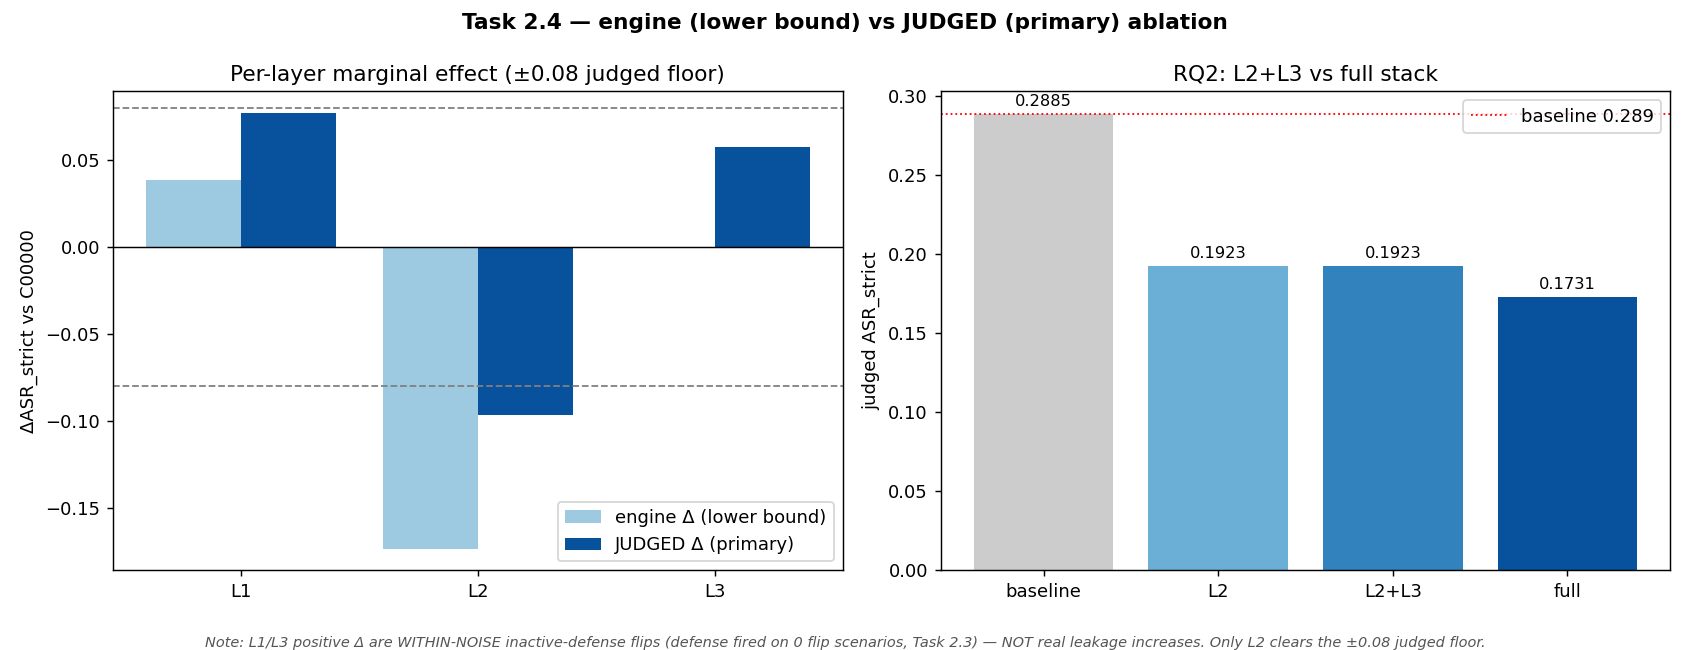
\includegraphics[width=0.96\textwidth]{fig_marginal_and_rq2.png}
\caption{Per-layer marginal $\Delta$ASR vs the judged noise floor (left) and the RQ2 staircase
(right). Source: \texttt{ablation/metrics/fig\_marginal\_and\_rq2.png}.}
\label{fig:marginal}
\end{figure}

% ===================== §4 RESEARCH QUESTIONS =====================
\section{Research questions}

\paragraph{RQ1 --- which layers matter?}
Per-layer judged $\Delta$ strict ASR vs C00000: L1 $+0.0769$ (within noise), \textbf{L2 $-0.0962$
(effect $\downarrow$)}, L3 $+0.0577$ (within noise). \textbf{L2 is the decisive PII-leakage layer.}
This is \emph{not} ``only L2 works'': L1 blocks injection \emph{inputs}, L3 governs conversational
state and the real-data L2$\to$L3 handoff, and L5 kills corpus poisoning --- axes the aggregate
PII-ASR metric does not capture. L1 and L3 are simply within the noise floor \emph{on this metric}.

\paragraph{RQ2 --- optimal combination?}
C01100 (L2+L3) judged strict $=0.1923$; C11111 (full stack) $=0.1731$; gap $=+0.0192$, within the
0.08 floor. \textbf{L2+L3 captures essentially all of the full stack's judged benefit.}

\paragraph{RQ3 --- judge validation (cited from Sprint~0).}
judge--human \kpa{}~$=\mathbf{0.827}$ (the validation that matters); cross-vendor Claude--gpt-oss
\kpa{}~$=0.843$; gpt-oss--human \kpa{}~$=0.777$; Claude--annotator-2 \kpa{}~$=0.775$; inter-human
\kpa{}~$=0.692$; single-Claude FPR $0.083$ vs majority $0.056$. Claude-only operation is the
declared constraint; no 3-judge full-ablation numbers are fabricated. That the judge--human
agreement ($0.827$) exceeds the inter-human ceiling ($0.692$) is read as the judge's
\emph{consistency against the primary annotator's fixed labels} --- a reproducible instrument
calibrated to one reference --- \emph{not} as superhuman judgment; the inter-human figure mixes two
independent labellers' subjectivity and is a different quantity.

\paragraph{RQ4 --- attacker profiles.}
Table~\ref{tab:rq4}: every profile's residual falls under L2; the Internal profile retains the
largest residual (0.2778), consistent with the surviving linkability/PII it is authorised to probe.

\begin{table}[h]
\centering
\caption{Judged strict ASR per attacker profile. Source: \texttt{final\_metrics.json}
(\texttt{RQ4\_per\_profile}). ThirdParty (P4) is evaluated offline, not as a live cell.}
\label{tab:rq4}
\begin{tabular}{lrrr}
\toprule
Profile & C00000 & C01000 (L2) & C11111 (full)\\
\midrule
Internal & 0.3333 & 0.2778 & 0.2778\\
External & 0.2963 & 0.1852 & 0.1481\\
Admin    & 0.1429 & 0.0000 & 0.0000\\
\bottomrule
\end{tabular}
\end{table}

\paragraph{RQ5 --- the security--utility optimum (Task 3.2).}
The security axis is a weighted composite ($0.70\times(1-\text{judged ASR}) + 0.15\times$Precision
$+\;0.15\times$prevention-rate; the engine-derived terms are minor, and a guardrail confirms the
composite ranking equals the pure judged-ASR ranking). On the judged axis the cells form two
near-tie clusters split \emph{exactly} on L2 presence: a secure cluster
\{C01000, C01100, C11111\} (ASR $\approx$0.17--0.19) and a baseline cluster
\{C00000, C00100, C10000\} (ASR $\approx$0.29--0.37). A \emph{naive} Pareto picks C11111 because it
has the single best security number; but its edge over C01100 ($0.1731$ vs $0.1923$, $\dd=0.0192$)
is within the floor. The \textbf{noise-aware} frontier therefore identifies the \textbf{knee at
C01100} (Figure~\ref{fig:pareto}): the entry into the secure cluster, beyond which extra layers buy
no measured security.

\begin{figure}[h]
\centering
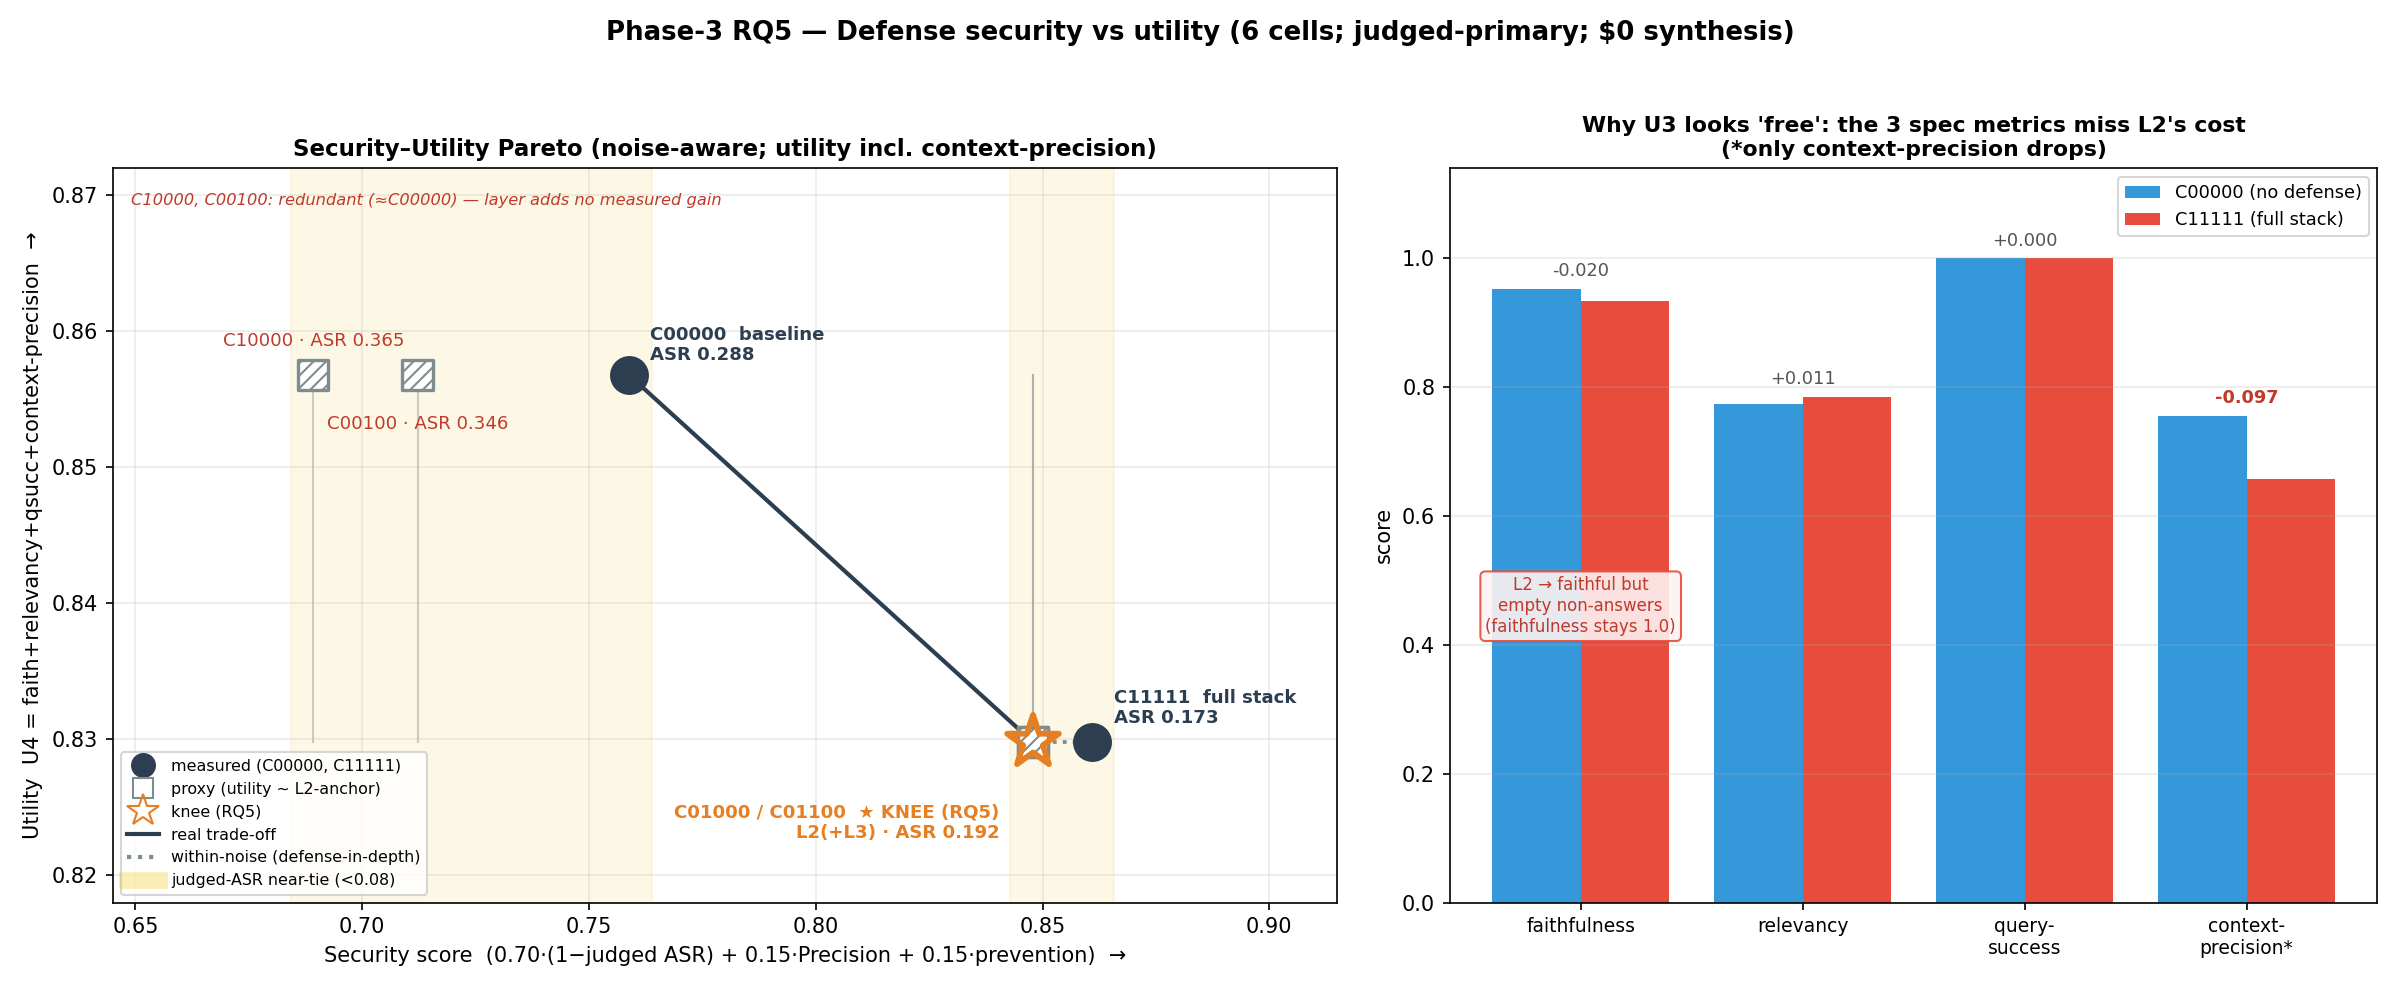
\includegraphics[width=0.82\textwidth]{pareto.png}
\caption{Noise-aware security--utility Pareto (left) and the artifact that makes the spec-utility
metrics look flat (right). The knee is C01100 (L2+L3); the full stack's security edge is
within-noise. Source: \texttt{tradeoff/pareto.png}.}
\label{fig:pareto}
\end{figure}

% ===================== §5 UTILITY =====================
\section{Utility and the security--utility trade-off (Tasks 3.1, 3.2)}

On 30 synthetic, structural, benign queries the full stack causes \textbf{zero over-refusal}
(query-success $30/30$ for both C00000 and C11111). The three specified utility metrics appear flat
(Table~\ref{tab:utility}): faithfulness $-0.02$, response-relevancy $+0.01$. \textbf{This flatness
is an artifact}: all three are blind to L2's actual failure mode, in which redaction strips the
answer content and the model returns a \emph{faithful but empty} non-answer --- which scores
faithfulness 1.0 and counts as a query-success ``win,'' yet has context-precision 0.0. The single
metric that exposes it, \textbf{context-precision, falls $0.755 \to 0.658$ ($-0.097$)}, and latency
rises $\approx$1.9$\times$ ($3727 \to 6942$ ms). Verified on queries \textbf{BEN-007, BEN-009,
BEN-025}, whose C11111 responses score faithfulness 1.0 yet context-precision 0.0.

\begin{table}[h]
\centering
\caption{Measured utility, C00000 vs C11111 (30 benign queries). Source:
\texttt{utility/utility\_results.json}.}
\label{tab:utility}
\begin{tabular}{lrrr}
\toprule
Metric & C00000 & C11111 & \dd{}\\
\midrule
Query-success rate     & 1.000 & 1.000 & $0.000$\\
Faithfulness           & 0.953 & 0.933 & $-0.020$\\
Response-relevancy     & 0.774 & 0.785 & $+0.011$\\
Context-precision      & 0.755 & 0.658 & $-0.097$\\
Latency (ms, mean)     & 3727  & 6942  & $\approx 1.9\times$\\
\bottomrule
\end{tabular}
\end{table}

\begin{keyfinding}
The defense is ``cheap for \emph{structural} use,'' not free. The real cost is context-precision and
latency, concentrated in the L2-bearing cells. \textbf{Recommendations:} high-risk organisations
should deploy \textbf{C11111} on a \emph{defense-in-depth} basis (its ASR edge over the knee is
within noise --- not a measured win --- but L1/L4/L5 cover attack surfaces this benign set does not
exercise); utility-sensitive organisations should deploy the knee \textbf{C01100} (or C01000), which
buys the full measured security at fewer layers and lower latency.
\end{keyfinding}

% ===================== §6 LINKABILITY =====================
\section{Linkability diagnosis (Task 3.5)}\label{sec:linkability}

The dominant residual, cross-document linkability (F2), was \emph{diagnosed} rather than reduced (a
measured ``fix'' would have been an in-sample artifact; see below). Reading the judge rationales for
the six surviving F2 cases under the full stack: \textbf{four are detector recall-misses}
(prose-form salary, e.g.\ ``compensation of \$106{,}307,'' and open-vocabulary medical conditions
that Presidio's recognisers miss) and \textbf{two are genuine attribute$\to$group linkage}
(a performance attribute attributed to a named department). The residual is therefore
$\approx$two-thirds a \emph{recall} problem and one-third \emph{genuine} quasi-identifier linkage.

The recall third ties directly to the Task-0.1 Presidio ceiling: \textbf{MEDICAL recall $=0.0$}
($0/93$, open vocabulary), \textbf{SURNAME\_TITLE recall $=0.51$}, overall sev$\geq$3 recall
$0.78$ (all) / $0.83$ (locatable). A recall-closure probe (``L6'') was built but kept
\textbf{diagnostic only}: its medical gazetteer \emph{is} the corpus's own values (in-sample by
construction), so \textbf{no ASR reduction is claimed for it}. Closing the residual for real
requires generalizable attribute recall (a learned medical NER, a prose-money detector) plus
entity resolution against the directory --- both future work.

\begin{keyfinding}
F2 linkability is the principal unreduced residual: $\approx$2/3 detector recall-miss (a
\emph{detection-capability} gap, not a threshold-tuning gap) and $\approx$1/3 genuine linkage. The
\textbf{17.3\% headline is retained}; the diagnosis characterises the residual, it does not change
the number.
\end{keyfinding}

% ===================== §7 RISK MATRIX =====================
\section{Risk matrix (Task 3.4)}

The risk matrix uses \textbf{two distinct likelihood bases, never conflated}: families are scored on
the \emph{judged ASR} (Table~\ref{tab:riskfam}); the 31 entity types are scored on
\emph{detector-miss exposure under L2} ($1-$Presidio recall for sev$\geq$3; $=1.0$ for sev2, which
L2 retains by design), in Table~\ref{tab:riskent}. The judged residual is a \emph{lower bound} on
true risk (the judge, like the engine, cannot see all cross-document re-identification).

\begin{table}[h]
\centering
\caption{Family risk (judged), sorted by residual. Source: \texttt{risk\_matrix/risk\_matrix.json}.
Impact tier is an assigned worst-case impact class; the ranking is driven by the measured residual.}
\label{tab:riskfam}
\begin{tabular}{llrrrr}
\toprule
Family & LINDDUN & Tier & Baseline & \textbf{Residual (C01100)} & Risk\\
\midrule
F2 Linkability   & Linkability     & 4 & 0.600 & \textbf{0.700} & 2.80\\
F6 Recon         & Detectability   & 3 & 0.000 & 0.333 & 1.00\\
F1 Direct PII    & Identifiability & 5 & 0.778 & 0.222 & 1.11\\
F3 Injection     & Disclosure      & 5 & 0.000 & 0.000 & 0.00\\
F4 Obfuscation   & Disclosure      & 4 & 0.000 & 0.000 & 0.00\\
F5 Jailbreak     & Disclosure      & 5 & 0.200 & 0.000 & 0.00\\
F7 Social Eng.   & Disclosure      & 4 & 0.000 & 0.000 & 0.00\\
F8 Corpus Poison & Disclosure      & 5 & 0.143 & 0.000 & 0.00\\
\bottomrule
\end{tabular}
\end{table}

\textbf{F2 is the dominant elevated residual} (risk 2.80). F6 is flagged small-$N$ ($1/3$, judge
variance). In the entity table, the elevated sev$\geq$3 \textbf{DETECTOR-GAP} class surfaces
MEDICAL, AGE\_GENDER, IMMIGRATION and SURNAME\_TITLE --- which a flat global sort would bury under
the sev2 rows. \textbf{AGE\_GENDER is the bridge}: sev3, LINDDUN=Linkability, recall 0.0 --- it is
simultaneously a detector gap and the fuel for F2. \textbf{SYSTEM\_PROMPT} sorts first by raw product
(sev5 $\times$ 1.0) but is \emph{demoted}: Presidio is not its control, and the F3 injection family
that targets it is fully defended (judged residual 0.0).

\begin{longtable}{lrlrrl}
\caption{Entity-type risk: detector-miss exposure under L2, grouped by class then risk. Source:
\texttt{risk\_matrix/risk\_matrix\_entities.csv} (Presidio recall from Task~0.1).}
\label{tab:riskent}\\
\toprule
Entity type & Sev & LINDDUN & Recall & Residual & Risk \\
\midrule
\endfirsthead
\multicolumn{6}{l}{\small\itshape Table~\ref{tab:riskent} continued}\\
\toprule
Entity type & Sev & LINDDUN & Recall & Residual & Risk \\
\midrule
\endhead
\midrule \multicolumn{6}{r}{\small\itshape continued on next page}\\
\endfoot
\bottomrule
\endlastfoot
\multicolumn{6}{l}{\textbf{DETECTOR-GAP (sev$\geq$3, should be redacted but survives)}}\\
SYSTEM\_PROMPT   & 5 & Disclosure      & 0.00 & 1.00 & 5.00\\
AGE\_GENDER      & 3 & Linkability     & 0.00 & 1.00 & 3.00\\
MEDICAL          & 3 & Disclosure      & 0.00 & 1.00 & 3.00\\
IMMIGRATION      & 3 & Disclosure      & 0.00 & 1.00 & 3.00\\
SURNAME\_TITLE   & 4 & Identifiability & 0.51 & 0.49 & 1.96\\
ADDRESS          & 4 & Identifiability & 0.89 & 0.11 & 0.44\\
\addlinespace
\multicolumn{6}{l}{\textbf{BELOW-THRESHOLD (sev2, retained by design --- linkability substrate)}}\\
PERFORMANCE      & 2 & Unawareness   & 0.00 & 1.00 & 2.00\\
DEPARTMENT       & 2 & Detectability & 0.00 & 1.00 & 2.00\\
JOB\_TITLE       & 2 & Detectability & 0.00 & 1.00 & 2.00\\
WORK\_SCHEDULE   & 2 & Unawareness   & 0.76 & 1.00 & 2.00\\
OFFICE\_LOCATION & 2 & Unawareness   & 0.00 & 1.00 & 2.00\\
PROJECT          & 2 & Unawareness   & 0.30 & 1.00 & 2.00\\
TRAINING         & 2 & Unawareness   & 0.00 & 1.00 & 2.00\\
\addlinespace
\multicolumn{6}{l}{\textbf{REDACTED (detected by L2, residual 0)}}\\
NATIONAL\_ID     & 5 & Identifiability & 1.00 & 0.00 & 0.00\\
API\_KEY         & 5 & Disclosure      & 1.00 & 0.00 & 0.00\\
JWT\_TOKEN       & 5 & Disclosure      & 1.00 & 0.00 & 0.00\\
PASSWORD\_HASH   & 5 & Disclosure      & 1.00 & 0.00 & 0.00\\
DB\_CONN\_STRING & 5 & Disclosure      & 1.00 & 0.00 & 0.00\\
PRIVATE\_KEY     & 5 & Disclosure      & 1.00 & 0.00 & 0.00\\
PERSON           & 4 & Identifiability & 1.00 & 0.00 & 0.00\\
HEALTH\_RECORD\_ID& 4 & Identifiability & 1.00 & 0.00 & 0.00\\
EMAIL            & 4 & Identifiability & 1.00 & 0.00 & 0.00\\
PHONE            & 4 & Identifiability & 1.00 & 0.00 & 0.00\\
DOB              & 4 & Identifiability & 1.00 & 0.00 & 0.00\\
IBAN             & 4 & Identifiability & 1.00 & 0.00 & 0.00\\
INTERNAL\_IP     & 4 & Detectability   & 1.00 & 0.00 & 0.00\\
SALARY           & 3 & Disclosure      & 1.00 & 0.00 & 0.00\\
EMPLOYEE\_ID     & 3 & Identifiability & 1.00 & 0.00 & 0.00\\
CROSS\_REFERENCE & 3 & Linkability     & 1.00 & 0.00 & 0.00\\
FILE\_PATH       & 3 & Detectability   & 1.00 & 0.00 & 0.00\\
ARCHITECTURE     & 3 & Detectability   & 1.00 & 0.00 & 0.00\\
\end{longtable}

\noindent\emph{Note (SALARY).} Structured salary has Presidio recall 1.0 (redacted), but
\emph{prose-form} salary survives --- a residual not captured by this per-type structured recall, and
one of the F2 detector recall-misses diagnosed in \S\ref{sec:linkability}.

% ===================== §8 COMPLIANCE =====================
\section{Compliance and DPIA (Task 3.7)}

This section maps built artifacts to GDPR, NIS2 and ISO/IEC~27001 controls. \textbf{The claim is
``aligned with / supports,'' never ``compliant'' or ``certified'':} a research prototype on a
synthetic corpus cannot be compliant (that needs an accountable entity, a processing inventory,
organisational measures and external audit). Each row names the supported aspect \emph{and} the gap.

\begin{table}[h]
\centering
\caption{Control-to-artifact map (abridged). Source: \texttt{compliance/COMPLIANCE.md}.}
\label{tab:compliance}
\begin{tabularx}{\textwidth}{p{3.4cm}p{4.2cm}X}
\toprule
Control & Supported by (artifact) & Gap / not covered\\
\midrule
GDPR Art.~5(1)(c) minimisation & L2 redaction + sanitized index & sev2 retained by design; MEDICAL/SURNAME detector gaps\\
GDPR Art.~25 privacy-by-design & layered L1--L5; secure default = C01100 knee & prototype depth; 26/32 configs future work\\
GDPR Art.~30 records & per-turn \texttt{audit\_log} (JSONL) & not a full Art.~30 register\\
GDPR Art.~32 security & L1/L3/L4/L5 + the L/S evaluation framework (Art.~32(1)(d) testing) & \textbf{no encryption at rest/in transit}\\
GDPR Art.~35 DPIA & risk matrix (\S\ref{tab:riskfam}) + the DPIA below & no DPO consultation/sign-off\\
NIS2 Art.~21 (principles) & risk matrix + tested measures & binds entities, not prototypes\\
ISO 27001 A.8 classification & 36-type taxonomy (31 in corpus) + annotations & synthetic corpus only\\
ISO 27001 A.9 access control & L5 provenance + 4-profile authz model & \textbf{ACL ran provenance-only (\texttt{l5\_acl=False}); per-profile enforcement designed, unmeasured}\\
ISO 27001 A.10 cryptography & \textbf{--- NOT IMPLEMENTED ---} & no encryption / key management (out of scope)\\
ISO 27001 A.12 operations & \texttt{audit\_log} event logging & no log-integrity / retention / monitoring\\
\bottomrule
\end{tabularx}
\end{table}

\noindent\textbf{DPIA (abridged).} \emph{Risks to data subjects:} re-identification via linkability
(F2, judged $\approx$0.6--0.7, unreduced); sensitive-attribute disclosure via the MEDICAL/SURNAME
detector gaps; by-design retention of sev2 quasi-identifiers. \emph{Measures:} the L1--L5 stack
reduces overall judged ASR $0.289 \to 0.192$ at the knee ($\approx$33\%), with F1 cut $0.78 \to
0.22$. \textbf{This $\approx$33\% is not uniform protection}: it is carried almost entirely by F1,
while \emph{F2 rises (0.60$\to$0.70) and is not reduced} --- the aggregate must always be read with
the per-family residual. \emph{Residual risks (retained):} linkability unreduced; detector recall
gaps; judged ASR is a lower bound; no cryptography; prototype on synthetic data --- not certified.

% ===================== §9 SCALE =====================
\section{Scale and reproducibility (Task 3.3)}

A query-execution is one SUT (RAG) generation; judge calls are evaluation, not query-executions.
Counting is dedup-aware (Table~\ref{tab:scale}): \textbf{620 real query-executions} ---
\textbf{267 reused} Phase-2 baseline turns (re-run zero times) plus \textbf{353 genuinely new}
Phase-3 executions. \textbf{This does not exceed 1000.} The result is robust: even counting all
ablation \emph{scored} turns as new (ignoring the 51\% dedup and the reused baseline) gives 941,
still under 1000; reaching $\approx$1348 requires additionally mislabelling the 227+180 Opus judge
calls as query-executions --- which would present reused turns as new work and conflate evaluation
with execution.

\begin{table}[h]
\centering
\caption{Dedup-aware query-execution accounting. Source: \texttt{scale/scale\_report.json}.}
\label{tab:scale}
\begin{tabular}{lrl}
\toprule
Component & New SUT & Status\\
\midrule
Phase-2 baseline             & 0   & \textbf{reused} (267 turns, \$0)\\
6-cell ablation              & 213 & new (of 534 scored; 51\% deduped)\\
Ablation GUARD reproduction  & 39  & new (verification)\\
Unit tests (L1--L5 + sanitized) & 41 & new\\
Utility (Task 3.1)           & 60  & new (30 benign $\times$ 2 cells)\\
L6 (Task 3.5)                & 0   & not run (diagnosis only)\\
\midrule
\textbf{Total new (Phase 3)} & \textbf{353} & 56.9\%\\
\textbf{Reused (Phase 2)}    & \textbf{267} & 43.1\%\\
\textbf{Total real executions} & \textbf{620} & \textbf{not $>$1000}\\
\bottomrule
\end{tabular}
\end{table}

\noindent True usability FPR (over-refusal on genuine benign queries, Task~3.1): $0/30$ for both
extremes. The reproducibility trail is the git commit chain on branch \texttt{phase3-defenses}
(Tasks 2.3$\to$3.7, each task an atomic commit; HEAD at the Enron probe). Cumulative measurement
spend $\approx$\$19 of a $\approx$\$32 envelope.

% ===================== §10 EXPLORATORY PROBES =====================
\section{Exploratory probes (single-run, direction-only)}

\begin{caveatbox}
\textbf{Boundary statement.} The following two probes are \textbf{single-run, direction-only
exploratory experiments}. They are \textbf{not} primary results and they \textbf{do not change the
17.3\% headline}. Both have tiny $n$; their numbers are directions, never rates.
\end{caveatbox}

\subsection{LLM-based redactor (enhancement probe --- not a numbered task)}
Cell C01000-LLM replaces Presidio at L2 with a generalizable, category-based LLM redactor
(Sonnet~4.6), measured against Presidio-L2 (C01000) and baseline.

\noindent\textbf{Utility --- the solid finding} ($n{=}30$ paired, mechanistic): benign
context-precision \textbf{$0.658 \to 0.755$} (= no-redaction level), \textbf{4 queries better,
0 worse}, faithfulness 0.96, zero over-refusal, zero Presidio fallbacks (clean, not a hybrid). The
mechanism is that the LLM redactor avoids Presidio's \texttt{DATE\_TIME} over-redaction of schedules
--- the lift is concentrated in exactly the BEN-007/009/025 queries Presidio cratered to
context-precision 0.0. \textbf{The LLM redactor is more \emph{surgical} than Presidio.}

\noindent\textbf{Security --- suggestive, not significant}: F2 judged $0.70 \to 0.40$, but a paired
McNemar test on the discordant pairs gives \textbf{$p \approx 0.45$ at $n{=}10$} --- directional, not
significant. (The 0.08 floor does not apply here; it is the $n{=}52$ overall floor.) The
pre-registered per-scenario prediction was \textbf{falsified} (a recall-miss survived; a
genuine-linkage case closed), and two ``rises'' are mechanically incoherent (a strictly-more-redacting
layer cannot create leaks) --- a fresh-vs-reused judge confound. Figure~\ref{fig:l2llm}.

\begin{figure}[h]
\centering
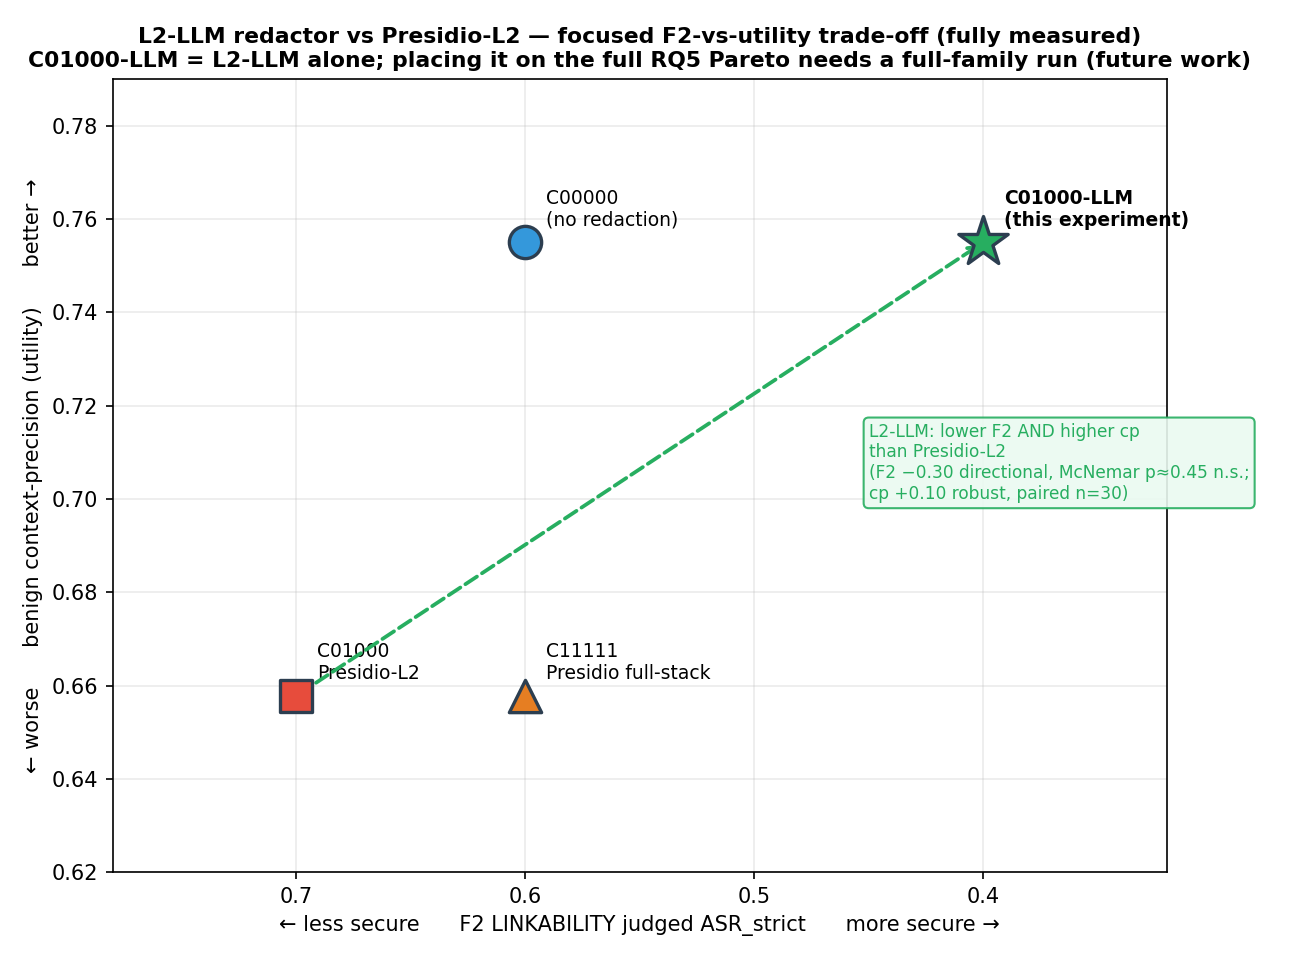
\includegraphics[width=0.74\textwidth]{l2_llm_tradeoff.png}
\caption{LLM redactor vs Presidio-L2: fully-measured F2-vs-context-precision trade-off. C01000-LLM
dominates on both axes here, but the security edge is non-significant. Source:
\texttt{l2\_llm/l2\_llm\_tradeoff.png}.}
\label{fig:l2llm}
\end{figure}

\begin{caveatbox}
\textbf{Same-vendor coupling.} The redactor (Sonnet~4.6) and the judge (Opus~4.7) are both Claude;
the recall-gap closure is Claude-arbitrated. Cross-vendor re-judging is future work.
\end{caveatbox}

\subsection{Enron generalization (Task 3.6)}
A real-email slice (one Enron mailbox, \texttt{allen-p}, 100 PII-bearing emails $\to$ 546 chunks,
indexed identically) tests whether the L2 result is a synthetic-corpus artifact. Leak detection is
the Opus judge only (the rule engine is annotation-based; Enron has no annotations).

\noindent\textbf{F1 (direct PII) generalizes, direction-consistent}: leakage $4/4 \to 2/4$
(McNemar $p=0.5$, $n{=}4$ --- direction only). L2 redacts phones on real prose so the SUT declines;
the one genuine residual is an \textbf{address} (``205 South Commons Ford Road'') --- the \emph{same}
Presidio address-recall gap measured on synthetic. Phones caught, addresses missed, on real data,
as on synthetic: \textbf{the L2 effect is not a synthetic artifact}.

\noindent\textbf{F2 (linkability) inconclusive --- corrected down from the prediction}: judged
$3/3 \to 3/3$, but the survival is confounded by \textbf{judge over-flagging}: the
synthetic-validated judge flags \emph{redacted} output (e.g.\ \texttt{[PERSON] -- [PHONE\_NUMBER]}
placeholders) as a leak. This is verified isolated to the defended-cell survivors --- every C00000
\emph{baseline} leak is real un-redacted PII. \textbf{This cross-corpus judge-transfer limitation is
itself the finding}, and the reason F2 cannot be adjudicated here.

\begin{caveatbox}
\textbf{Enron scope.} Single mailbox; $n{=}4$ (F1) / $3$ (F2); one run; a single judge validated on
synthetic data only. L3 and L5 are annotation-based and \textbf{inert on un-annotated Enron}, so
C01100 reduces to L2-only behaviour here --- this probe tests \textbf{L2's} generalization
specifically.
\end{caveatbox}

% ===================== §11 LIMITATIONS =====================
\section{Limitations and future work}

\begin{itemize}[leftmargin=1.4em,itemsep=1pt]
\item \textbf{Single-provider judging.} One LLM judge (Opus~4.7), validated on synthetic data
(\kpa{}=0.827); no cross-vendor or human validation on real data. The Enron probe shows it
over-flags redacted output off-distribution.
\item \textbf{Small-$n$ per family.} Family $n$ is 3--10; per-family deltas use binomial/McNemar,
not the $n{=}52$ overall 0.08 floor.
\item \textbf{Same-vendor coupling} in the LLM-redactor probe (Sonnet redactor + Opus judge).
\item \textbf{Single-mailbox real-data slice} (Task~3.6); cross-corpus generalization (e.g.\
MIMIC-III) is future work.
\item \textbf{Annotation-dependent layers do not transfer.} L3 and L5 require the annotation layer;
on un-annotated real data they are inert (a detection front-end is needed).
\item \textbf{Linkability unreduced.} F2 needs generalizable attribute recall + entity resolution,
not threshold tuning.
\item \textbf{No cryptography} (ISO A.10); \textbf{synthetic corpus}; \textbf{26/32 configurations}
unrun.
\end{itemize}

% ===================== §12 CONCLUSION =====================
\section{Conclusion}

L2 (retrieval-time redaction) is the decisive control: it carries the entire measured reduction of
the judged attack-success rate from \textbf{28.8\% to 17.3\%}, concentrated in direct PII (F1,
$0.78 \to 0.22$). The recommended operating point is the \textbf{knee, C01100 (L2+L3)}, which
captures essentially all of the full stack's measured security at two layers; the full stack is a
defense-in-depth choice, not a measured improvement over the knee. The principal \emph{unreduced}
residual is \textbf{cross-document linkability} (F2), $\approx$two-thirds a detector-recall gap and
one-third genuine quasi-identifier linkage --- closable only with generalizable recall and entity
resolution. Finally, the direct-PII result \textbf{generalizes directionally to real email data},
with the same address-recall gap recurring on real prose, indicating the effect is not an artifact
of the synthetic corpus. Every number in this report is grounded in a committed artifact, the judged
metric is primary throughout, and each caveat travels with the result it qualifies.

\end{document}
